\section{Documentation}
In order for SINATRA to be used by other users and developers, the code must be well documented. It is important to have systems of documentation in place for all of the different levels of instructions, guidelines, comments, and information. The documentation  can be broken into two sections; for the user and for the developer. These systems must be simple, reliable, clear, and resilient. The goal is to make the code easy to distribute, simple to learn to the level necessary, and for the changes, bugs, and suggestions to be centralized.

\subsection{GitHub}
The system chosen to organize and host SINATRA for developers is GitHub. Github is an online file storage, syncing, and collaboration work space for developing code bases. It is easy to use, popular, and therefore support for using it is strong. SINATRA is housed on GitHub by the author and is shared with Dr. Amelia Greig and Dr. David Marshall. On account of the code’s license the repository is private and developers can get access by contacting the Aerospace Department at Cal Poly, SLO. \par
\indent GitHub has three major features used in SINATRA: the commits system, the branches system, and the ReadME files. The commits system is a method of allowing multiple developers to work on the same code base without breaking the other developers builds. Each developer works on the code on their local machines and once they have a stable addition to SINATRA, they commit it to the GitHub where it is merged into the current version. Whenever other users are working, they can pull those changes on to their local machine. This helps development moved along smoothly, although it does require communication between the developers to ensure they are not working on the same lines of code and creating different outcomes. This commit structure also allows the code base to be version controlled, which helps with mistakes, reverting to older versions, and following the change logs. \par


\begin{figure}
\includegraphics[width=.95\textwidth]{branching.png}
\centering
\caption{Example of GitHub workflow}
\label{fig:github}
\end{figure}




\indent Another feature of GitHub utilized during the development of SINATRA was the branches feature. Branches allow a user to create a separate branch of the code base. An example workflow can be seen in Figure \ref{fig:github}. As shown, there is a "master" branch which holds the current official version. When a developer wants to build a new feature, they create a "branch" of the code. On that branch they develop the feature so that the master can continue to be used for official uses. Once the feature is complete the developer submits a "pull" request which shows the feature and resulting changes to the "master" branch. The team then approves the feature and it is merged into the official "master" branch. Branches are used to develop a large new section of code with the features and security of GitHub and without cluttering the teams main code with testing and validation edits. This process allows developers to command their own section of the code, update and test, and then make it available for the other developers to work with. This ensures a constant work flow where multiple developers can work on different features and not have to worry about whether their testing and tinkering will hinder others’ work on the master branch. In this way the development continues without bottlenecks, nor need for constant communication between the developers. \par


\indent The final feature used in GitHub was the ReadME files. These files are automatically displayed by GitHub’s system when you enter the directory. This allows the developers to convey how that directory fits into the code base, and specifics on the files in the directory, and instructions on how to use the directory. The author has outfitted all of SINATRA’s directories with ReadME files. These features were the reason that the author choose GitHub to host SINATRA and they were utilized during development in order to allow efficient and clear code creation. SINATRA's main ReadME page is shown in Figure \ref{fig:readme}, as shown on GitHub's website. 

\begin{figure}
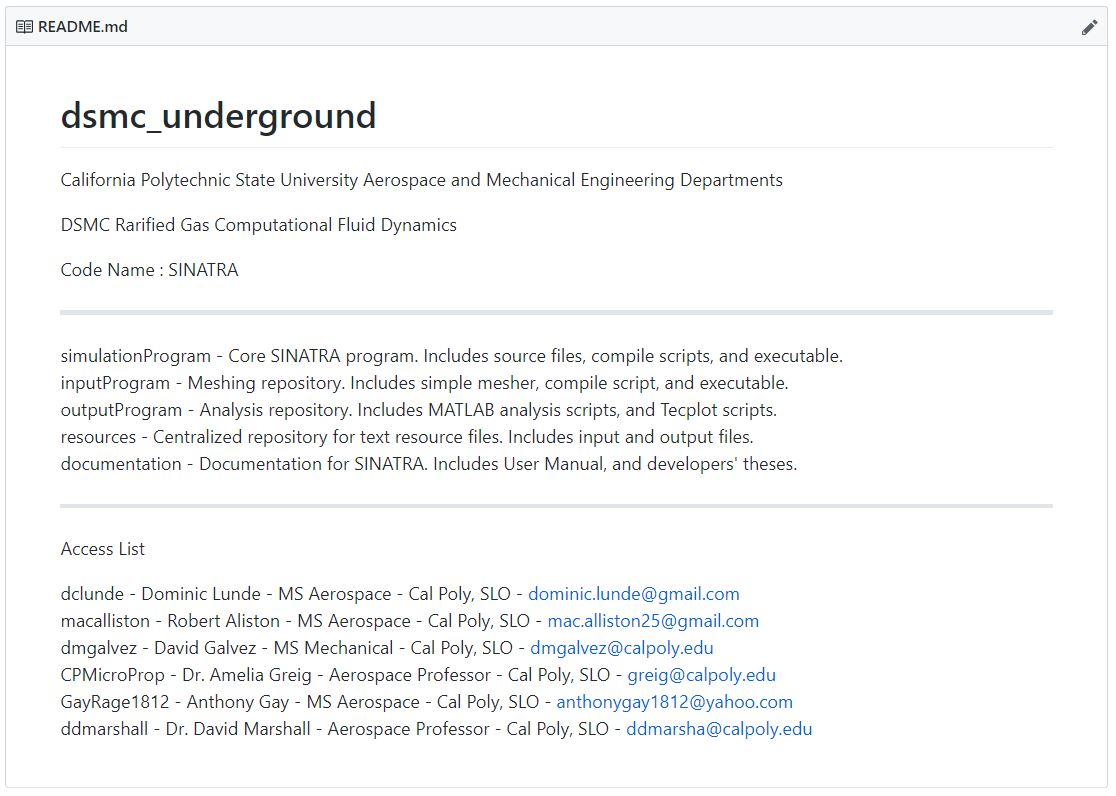
\includegraphics[width=.95\textwidth]{Readme.JPG}
\centering
\caption{SINATRA's main ReadME page}
\label{fig:readme}
\end{figure}


\subsection{Doxygen}
Doxygen is an automatic documentation creator from source code \footnote{Doxygen:  Main Page - \url{http://www.doxygen.nl/}}. It was chosen, configured, and used to create the SINATRA Developer Manual. Doxygen is given access to the source code, which it searches through and creates comprehensive documentation of the code base. For SINATRA, it creates descriptions of all of the classes, functions, and files. It shows what each class consists of. For example, it shows that the Mesh class contains structure classes, public types, public member functions and more as seen in Figure \ref{fig:Doxygen_Mesh}. It is built in HTML so each attribute is linked to the actual function. It is also possible to see the location of that item in the source code. \par

% to do talk about how simple it is to comment

\indent The important part of Doxygen is that it allows the user to customize the documentation. It allows the HTML file to be built in many different ways to make it work best for SINATRA. But more importantly, it takes comments made in the source code about the attributes and displays them in a clear and concise way. This allows a developer to quickly find an attribute where it is referenced in the rest of the source code, where it is built, and what the creator commented about it. This allows new developers to quickly learn SINATRA and start developing their own features. It also allows quick debugging of heritage code by new developers, which ensures that SINATRA will not fall victim to an error that can only be reasonably fixed by the original developer. The author has created a Doxygen manual of SINATRA, as well as a Doxygen input file and batch script for easily updating the manual as more developers add to SINATRA. See Appendix \ref{app:doxygenlists} for a list of all classes and files in SINATRA which have been commented with Doxygen. This is not a comprehensive guide to exactly what each function and variable does, but the author has commented every function in SINATRA to guide new developers.


\begin{figure}
\includegraphics[width=.95\textwidth]{Doxygen_Mesh.png}
\centering
\caption{Documentation created by Doxygen for the Mesh Class}
\label{fig:Doxygen_Mesh}
\end{figure}


\subsection{User Distribution}

As mentioned above, Github will be the primary source of distribution for developers of SINATRA. However, for less serious users, there is a simple distribution. It includes the mesh and simulation executables and input files. It also includes the GUI executable and finally a simple Matlab analysis script to visualize the particles. It has documentation which guides the user through a simple test case and show the user how the parts work together. This walk through can be found in Appendix \ref{app:walkthrough}. This distribution is packaged up in a zip file. The executables and other parts will only work on a Windows computer. Mac capability can be built through the source code and compiled on a Mac OS machine. \par

\indent This zip file can be sent to students for them to try simple test cases and produce new results. This distribution, while very simple and light in terms of file count, is actually a nearly full distribution of SINATRA. Almost all functions of the SINATRA work without the rest of the file structure and other code, therefore, it can be used for things such as the Bishop cluster to ensure the correct version of the code is being used. This allows a more direct way of controlling the simulation in new environments; however, it does exclude much of the functionality found within the actual code base itself. There are many test cases and options which can be activated in the source code. This distribution can be used to distribute and share SINATRA with relevant parties who want to produce DSMC results.
